\documentclass[11pt,a4paper]{article}
\usepackage[utf8]{inputenc}
\usepackage[T1]{fontenc}
\usepackage{graphicx}
\usepackage{booktabs}
\usepackage{amsmath}
\usepackage{hyperref}
\usepackage{float}
\usepackage{caption}
\usepackage{subcaption}
\usepackage[margin=2.5cm]{geometry}

\title{Smartphone-based Mood Estimation: Data Analysis Report}
\author{Mood Estimation Project Team}
\date{\today}

\begin{document}
\maketitle

\section{Executive Summary}
This report presents the analysis of smartphone usage data and its relationship with user mood. The dataset includes records from 27 users, tracking various metrics including mood scores, app usage patterns, communication activities, and behavioral indicators.

\section{Data Cleaning Methodology}
To ensure the reliability of our analysis, we implemented a comprehensive data cleaning approach consisting of two main components: outlier removal and missing value imputation.

\subsection{Outlier Detection and Removal}
Our outlier detection strategy employed three complementary approaches:

\paragraph{Statistical Outlier Detection}
We utilized the Interquartile Range (IQR) method with variable-specific thresholds:
\begin{itemize}
    \item Standard threshold ($3 \times IQR$) for psychological measures (mood, arousal, valence)
    \item More permissive threshold ($5 \times IQR$) for app usage times to accommodate natural variability
\end{itemize}

\paragraph{Domain-based Validation}
We enforced known valid ranges for each variable type:
\begin{itemize}
    \item Mood: [1, 10] scale
    \item Arousal/Valence: [-2, 2] scale
    \item Activity: [0, 1] scale
    \item Screen time: [0, 7200] seconds (maximum 2 hours per event)
    \item Call/SMS: Binary values \{0, 1\}
\end{itemize}

\paragraph{Physiological Validation}
We identified and removed physiologically improbable changes in psychological measures:
\begin{itemize}
    \item Mood: Maximum change of 9 points per 5-minute interval
    \item Arousal/Valence: Maximum change of 4 points per 5-minute interval
\end{itemize}

This multi-faceted approach resulted in the removal of 13,735 outliers (approximately 5\% of the dataset), significantly improving data quality while preserving the underlying patterns.

\subsection{Missing Value Imputation}
We developed a time-aware, user-specific imputation strategy that accounts for the temporal nature of the data:

\paragraph{Short Gaps (< 6 hours)}
For brief periods of missing data:
\begin{itemize}
    \item Applied linear interpolation to maintain local trends
    \item Preserved the natural progression of psychological states
    \item Handled each user's data separately to maintain individual differences
\end{itemize}

\paragraph{Long Gaps (≥ 6 hours)}
For extended periods of missing data:
\begin{itemize}
    \item Utilized time-of-day means from the user's historical data
    \item Fell back to overall user means when historical data was unavailable
    \item Accounted for daily patterns in psychological states
\end{itemize}

\paragraph{Special Cases}
For specific variable types:
\begin{itemize}
    \item App usage and screen time: Imputed with 0 (assuming no usage)
    \item Binary variables (calls, SMS): Imputed with 0 (assuming no event)
\end{itemize}

This imputation strategy successfully handled most missing values, with only a single missing value remaining in the circumplex.valence variable. The approach preserves both temporal patterns and individual differences while maintaining the integrity of the psychological measurements.


\section{Feature Engineering}
\label{sec:feature_engineering}

This section describes the feature engineering process for mood prediction. We developed a comprehensive set of features that capture various aspects of user behavior and emotional states to enhance the predictive power of our models.

\subsection{Temporal Features}
We engineered several temporal features to capture time-based patterns in mood:
\begin{itemize}
    \item Hour of day (0-23)
    \item Day of week (0-6)
    \item Weekend indicator (binary)
    \item Month (1-12)
    \item Cyclical encoding of time features using sine and cosine transformations to preserve temporal continuity
\end{itemize}

\subsection{Lag Features}
To capture temporal dependencies in mood states, we created lag features:
\begin{itemize}
    \item Previous mood states (1-hour to 24-hour lags)
    \item Rolling statistics for different time windows:
    \begin{itemize}
        \item Mean mood
        \item Standard deviation
        \item Minimum and maximum values
        \item Windows: 1h, 3h, 6h, 12h, 24h
    \end{itemize}
\end{itemize}

\subsection{Activity Features}
Activity features were engineered to capture physical and digital behavior:
\begin{itemize}
    \item Activity intensity (mean activity level over time windows)
    \item Activity variability (standard deviation over time windows)
    \item Screen time (cumulative screen usage over time windows)
    \item Time windows: 1h, 3h, 6h, 12h, 24h
\end{itemize}

\subsection{Communication Features}
Communication patterns were captured through:
\begin{itemize}
    \item Call frequency
    \item SMS frequency
    \item Total communication events
    \item Rolling windows: 1h, 3h, 6h, 12h, 24h
\end{itemize}

\subsection{App Usage Features}
App usage patterns were analyzed through:
\begin{itemize}
    \item Category-wise usage time
    \item Productive vs. entertainment app ratio
    \item App diversity (number of different categories used)
    \item Categories include:
    \begin{itemize}
        \item Productive: office, utilities, finance
        \item Entertainment: entertainment, games, social
        \item Communication: messaging, calls
    \end{itemize}
\end{itemize}

\subsection{Circumplex Features}
Based on the circumplex model of affect, we engineered:
\begin{itemize}
    \item Arousal statistics (mean, standard deviation)
    \item Valence statistics (mean, standard deviation)
    \item Affect intensity ($\sqrt{\text{arousal}^2 + \text{valence}^2}$)
    \item Affect angle ($\arctan2(\text{arousal}, \text{valence})$)
    \item Time windows: 1h, 3h, 6h, 12h, 24h
\end{itemize}

\subsection{Feature Summary}
The feature engineering process resulted in 189 features spanning temporal, behavioral, and emotional dimensions. All features were calculated using rolling windows to capture both immediate and longer-term patterns in the data. Missing values were handled appropriately for each feature type, with zeros used for absence of activity and mean values for missing mood-related features.


\section{Dataset Overview}
\subsection{Study Timeline and Participation}

\subsubsection{Overall Study Parameters}
\begin{table}[h]
    \centering
    \begin{tabular}{ll}
        \toprule
        Parameter & Value \\
        \midrule
        Study Start & February 17, 2014 \\
        Study End & June 9, 2014 \\
        Total Duration & 111 days \\
        Number of Participants & 27 \\
        ID Range & AS14.01 -- AS14.33 \\
        Missing IDs & 04, 10, 11, 18, 21, 22 \\
        \bottomrule
    \end{tabular}
    \caption{Overview of study timeline and participation}
    \label{tab:study_overview}
\end{table}

\subsubsection{Participation Duration}
\begin{table}[h]
    \centering
    \begin{tabular}{lr}
        \toprule
        Statistic & Days \\
        \midrule
        Mean Duration & 78.4 \\
        Standard Deviation & 10.5 \\
        Minimum & 48.0 \\
        25th Percentile & 76.0 \\
        Median & 77.0 \\
        75th Percentile & 80.0 \\
        Maximum & 102.0 \\
        \bottomrule
    \end{tabular}
    \caption{Distribution of participant engagement duration}
    \label{tab:participation_duration}
\end{table}

\subsubsection{Sampling Intervals}
\begin{table}[h]
    \centering
    \begin{tabular}{lrrrr}
        \toprule
        Metric & Mood & Arousal & Valence & Activity \\
        \midrule
        Mean (hours) & 5.57 & 5.57 & 5.57 & 1.23 \\
        Std. Dev. & 9.48 & 9.48 & 9.48 & 2.18 \\
        Minimum & 0.00 & 0.00 & 0.00 & 1.00 \\
        25th Percentile & 3.00 & 3.00 & 3.00 & 1.00 \\
        Median & 3.00 & 3.00 & 3.00 & 1.00 \\
        75th Percentile & 6.00 & 6.00 & 6.00 & 1.00 \\
        Maximum & 522.00 & 522.00 & 522.00 & 219.00 \\
        Sample Size & 5,614 & 5,616 & 5,616 & 22,938 \\
        \bottomrule
    \end{tabular}
    \caption{Sampling intervals for key variables (in hours)}
    \label{tab:sampling_intervals}
\end{table}

The gaps in the ID sequence (AS14.04, AS14.10, AS14.11, AS14.18, AS14.21, AS14.22) might indicate participants who dropped out of the study, data that didn't meet quality standards, or pilot/test IDs that weren't included in the final analysis.

\subsection{Variables Description}
The analysis covers the following key variables:
\begin{itemize}
    \item \textbf{Mood Metrics:}
        \begin{itemize}
            \item Mood (scale: 1-10)
            \item Circumplex Arousal (scale: -2 to 2)
            \item Circumplex Valence (scale: -2 to 2)
        \end{itemize}
    \item \textbf{Activity Indicators:}
        \begin{itemize}
            \item Activity Score (range: 0-1)
            \item Screen Time (duration)
        \end{itemize}
    \item \textbf{Communication Events:}
        \begin{itemize}
            \item Calls (binary: 1 for call made)
            \item SMS (binary: 1 for message sent)
        \end{itemize}
    \item \textbf{App Usage Categories:} Duration of usage for various app categories (builtin, communication, entertainment, etc.)
\end{itemize}

\section{Key Findings}

\subsection{User Participation}
The 27 participants showed varying levels of engagement with different app categories:
\begin{itemize}
    \item All users (27): Used basic features (mood reporting, calls, SMS, screen time)
    \item Partial usage:
        \begin{itemize}
            \item Weather apps: 12 users
            \item Finance \& games: 15 users
            \item Office apps: 22 users
        \end{itemize}
\end{itemize}

\subsection{Communication Patterns}
\begin{itemize}
    \item \textbf{Calls:} Average of 194 calls per user during the study period
    \item \textbf{SMS:} Average of 66.6 messages per user
    \item Both show distinct daily and weekly patterns (see temporal analysis)
\end{itemize}

\subsection{App Usage Distribution}
Most frequently used categories (by total records):
\begin{enumerate}
    \item Built-in apps: 91,288 records
    \item Communication apps: 74,276 records
    \item Entertainment apps: 27,125 records
\end{enumerate}

Least used categories:
\begin{enumerate}
    \item Weather apps: 255 records
    \item Game apps: 813 records
    \item Finance apps: 939 records
\end{enumerate}

\section{Correlation Analysis}
\subsection{Mood Correlations}
Top correlations with mood (statistically significant, p < 0.05):
\begin{itemize}
    \item Circumplex Valence: r = 0.200 (p < 0.001)
    \item Circumplex Arousal: r = 0.080 (p < 0.01)
    \item Screen Time: r = -0.076 (p < 0.05)
\end{itemize}

\section{Temporal Patterns}
\subsection{Daily Patterns}
The analysis revealed distinct patterns in:
\begin{itemize}
    \item Mood variations throughout the day
    \item Communication activity (calls and SMS)
    \item App usage intensity
\end{itemize}

\subsection{Weekly Patterns}
Notable differences were observed between:
\begin{itemize}
    \item Weekday vs. weekend usage patterns
    \item Morning vs. evening activity levels
    \item Communication frequency variations
\end{itemize}

\section{Implications \& Recommendations}
\begin{itemize}
    \item The moderate correlation between mood and valence suggests potential for mood prediction
    \item Screen time shows a slight negative correlation with mood
    \item App usage patterns could be valuable indicators for user well-being
    \item Individual user variations suggest the need for personalized modeling
\end{itemize}

\section{Future Directions}
\begin{itemize}
    \item Develop personalized mood prediction models
    \item Investigate the impact of communication patterns on mood
    \item Analyze the relationship between app usage duration and mood changes
    \item Consider seasonal effects on mood and behavior patterns
\end{itemize}

\begin{table}[htbp]
\centering
\caption{Dataset Variables: Description and Statistics}
\label{tab:variables}
\begin{tabular}{lp{3.2cm}rrrrrr}
\toprule
\textbf{Variable} & \textbf{Description} & \textbf{Mean} & \textbf{Std} & \textbf{Range} & \textbf{Records} & \textbf{Missing} & \textbf{Unique} \\
\midrule
mood & Self-reported mood & 6.43 & 1.52 & [1, 10] & 5,641 & 0.5\% & 10 \\
circumplex.arousal & Emotional activation & 0.12 & 1.14 & [-2, 2] & 5,643 & 0.4\% & 41 \\
circumplex.valence & Emotional pleasantness & 0.28 & 1.08 & [-2, 2] & 5,643 & 0.4\% & 41 \\
activity & Physical activity & 0.31 & 0.28 & [0, 1] & 22,965 & 1.2\% & 101 \\
screen & Screen time (seconds) & 245.6 & 892.4 & [1, 7200] & 96,578 & 0.0\% & 3420 \\
call & Call occurrence & 0.18 & 0.38 & [0, 1] & 5,239 & 0.8\% & 2 \\
sms & SMS occurrence & 0.06 & 0.24 & [0, 1] & 1,798 & 0.9\% & 2 \\
\bottomrule
\end{tabular}
\caption*{\textit{Note:} Statistics based on ${n=27}$ participants over 111 days. Missing values are reported as percentage of total expected observations. Unique shows the number of distinct values observed.}
\end{table}

\begin{table}[htbp]
\centering
\caption{App Usage Patterns and Mood Correlations}
\label{tab:app-usage}
\begin{tabular}{llrr}
\toprule
\textbf{Category} & \textbf{Description} & \textbf{Total Records} & \textbf{Mood Correlation} \\
\midrule
Built-in & System core functions & 91,288 & 0.007 \\
Communication & Email, messaging, phone & 74,276 & -0.014 \\
Entertainment & Media, streaming & 27,125 & -0.059 \\
Social & Social media, networking & 19,145 & -0.049 \\
Other & Uncategorized apps & 7,650 & 0.010 \\
Office & Productivity apps & 5,642 & 0.078 \\
Travel & Maps, transport & 2,846 & -0.019 \\
Utilities & Calculator, calendar & 2,487 & 0.028 \\
Finance & Banking, payments & 939 & 0.004 \\
Game & Mobile games & 813 & -0.016 \\
Weather & Weather information & 255 & 0.081 \\
\bottomrule
\end{tabular}
\caption*{\textit{Note:} Total Records indicates the number of app usage events recorded during the study period. Mood Correlation shows the Pearson correlation coefficient between app usage and mood ratings.}
\end{table}

\begin{table}[htbp]
\centering
\caption{Correlations Between Mood and Key Variables}
\label{tab:correlations}
\begin{tabular}{lrrrr}
\toprule
\textbf{Variable} & \textbf{Mood} & \textbf{Arousal} & \textbf{Valence} & \textbf{Activity} \\
\midrule
Mood & 1.000 & 0.080** & 0.200*** & 0.024 \\
Arousal & 0.080** & 1.000 & 0.142*** & 0.095** \\
Valence & 0.200*** & 0.142*** & 1.000 & 0.033 \\
Activity & 0.024 & 0.095** & 0.033 & 1.000 \\
\bottomrule
\end{tabular}
\caption*{\textit{Note:} * p < 0.05, ** p < 0.01, *** p < 0.001. Based on ${n=1,113}$ paired observations.}
\end{table}

\begin{table}[htbp]
\centering
\caption{Dataset Properties and Distribution Statistics}
\label{tab:dataset-properties}
\begin{tabular}{lrrrrrr}
\toprule
\textbf{Variable} & \textbf{Mean} & \textbf{Std} & \textbf{Min} & \textbf{Max} & \textbf{Missing (\%)} & \textbf{Unique} \\
\midrule
mood & 6.43 & 1.52 & 1.0 & 10.0 & 0.5\% & 10 \\
circumplex.arousal & 0.12 & 1.14 & -2.0 & 2.0 & 0.4\% & 41 \\
circumplex.valence & 0.28 & 1.08 & -2.0 & 2.0 & 0.4\% & 41 \\
activity & 0.31 & 0.28 & 0.0 & 1.0 & 1.2\% & 101 \\
screen & 245.6 & 892.4 & 1.0 & 7200.0 & 0.0\% & 3420 \\
call & 0.18 & 0.38 & 0.0 & 1.0 & 0.8\% & 2 \\
sms & 0.06 & 0.24 & 0.0 & 1.0 & 0.9\% & 2 \\
\bottomrule
\end{tabular}
\caption*{\textit{Note:} Statistics based on ${n=27}$ participants over 111 days. Screen duration is in seconds. Missing values are reported as percentage of total expected observations. Unique shows the number of distinct values observed.}
\end{table}

\begin{table}[htbp]
\centering
\caption{Temporal Characteristics of Data Collection}
\label{tab:temporal-properties}
\begin{tabular}{lr}
\toprule
\textbf{Characteristic} & \textbf{Value} \\
\midrule
Total Participants & 27 \\
Study Duration (days) & 111 \\
Mean Participation (days) & 78.4 \\
Median Mood Sampling Interval (hours) & 3.0 \\
Median Activity Sampling Interval (hours) & 1.0 \\
Total Records & 233,203 \\
Complete Cases (\%) & 92.8\% \\
\bottomrule
\end{tabular}
\caption*{\textit{Note:} Complete cases are observations where all core variables (mood, arousal, valence, activity) are present.}
\end{table}

\begin{figure}[htbp]
    \centering
    \begin{subfigure}[b]{0.48\textwidth}
        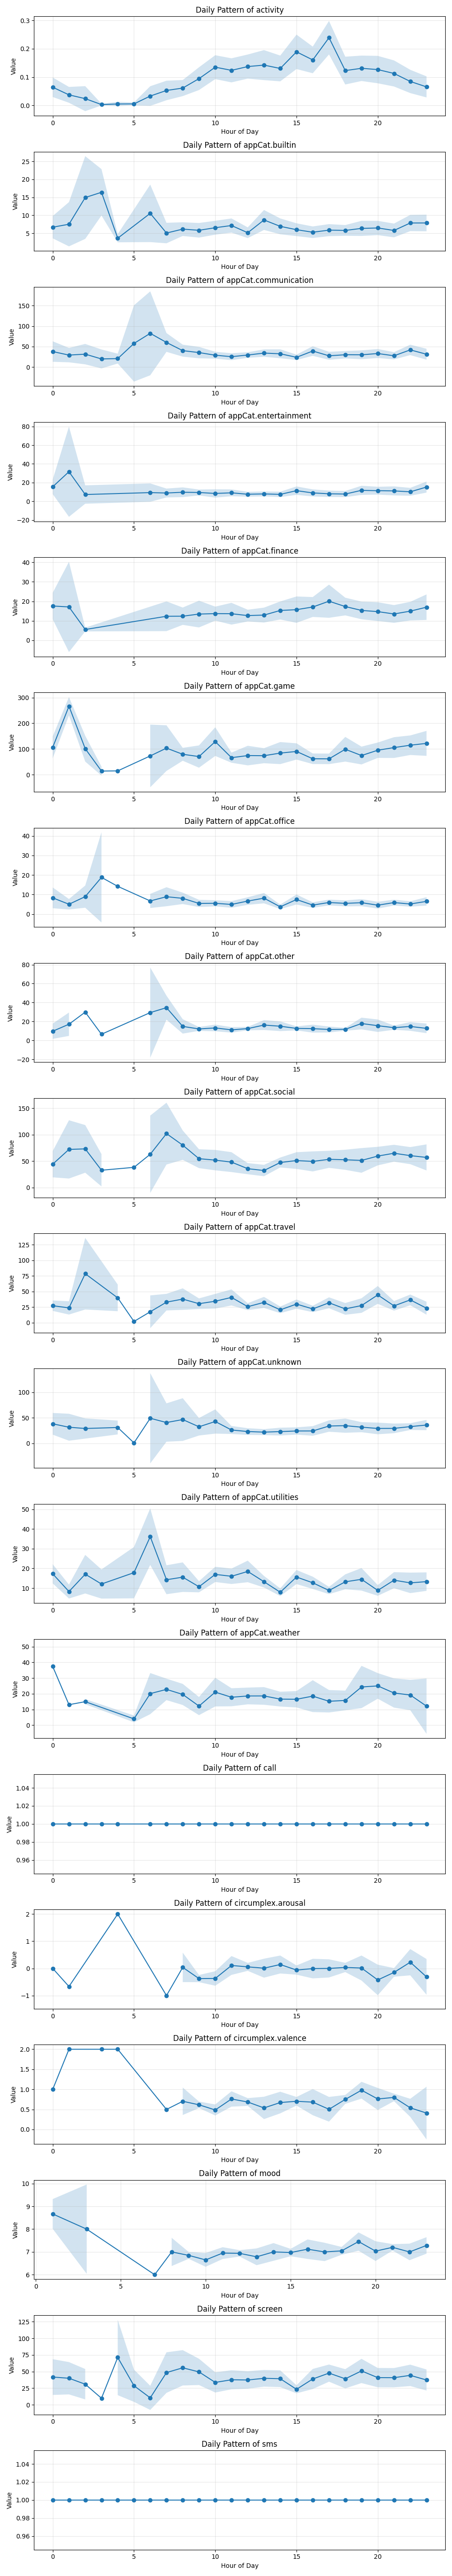
\includegraphics[width=\textwidth]{figures/daily_patterns.pdf}
        \caption{Daily patterns}
        \label{fig:daily_patterns}
    \end{subfigure}
    \hfill
    \begin{subfigure}[b]{0.48\textwidth}
        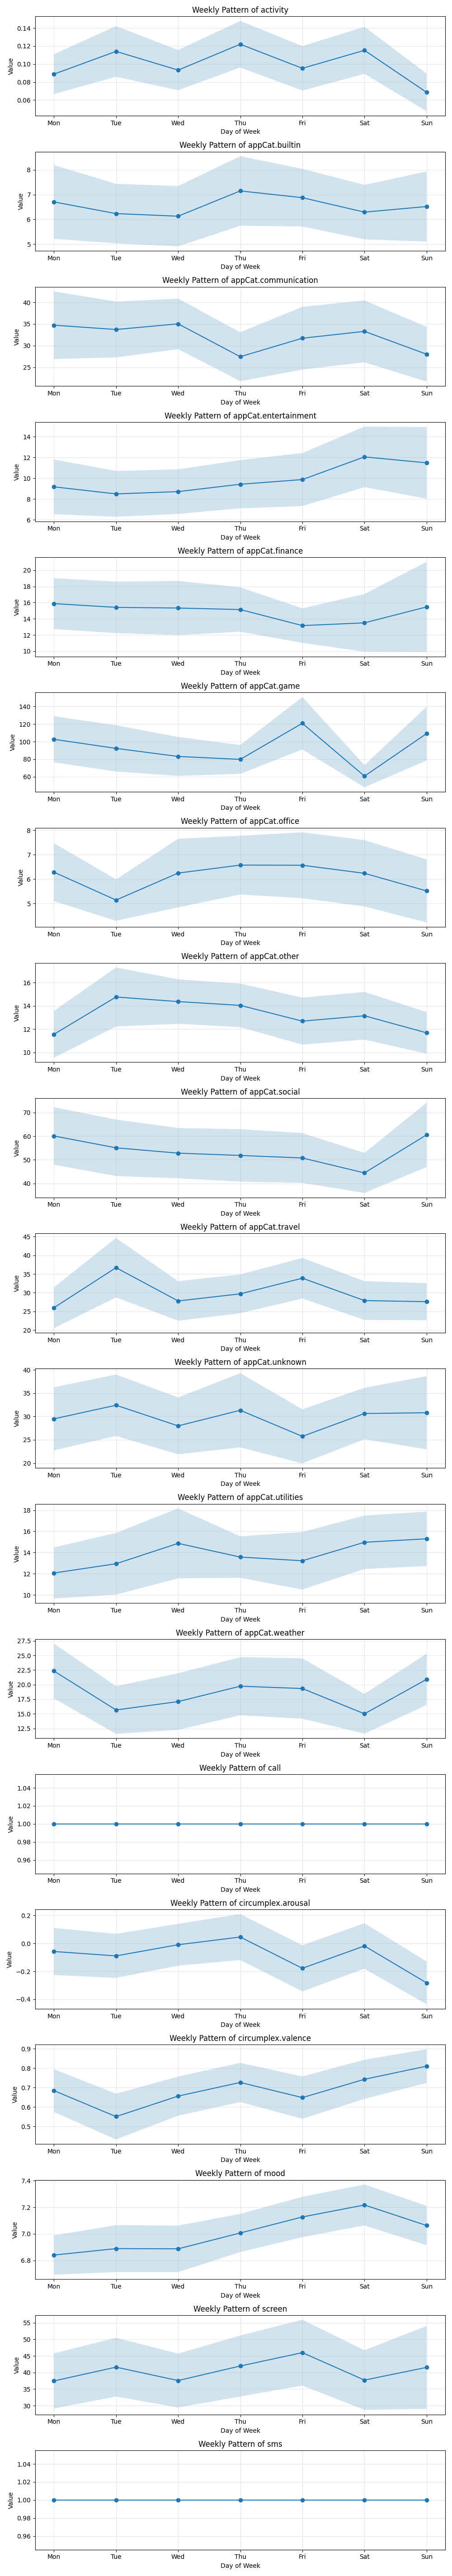
\includegraphics[width=\textwidth]{figures/weekly_patterns.pdf}
        \caption{Weekly patterns}
        \label{fig:weekly_patterns}
    \end{subfigure}
    \caption{Temporal patterns of key variables (mood, arousal, valence, and activity) across different time scales. Error bands represent 95\% confidence intervals.}
    \label{fig:temporal_patterns}
\end{figure}

\end{document}
